\chapter{Post-Darwin evidences of natural selection and evolution (I)}

%% some doubts about natural selection \cite{Ridley}
The role of the notion of epigenetics in the Modern Synthesis \cite{Baedke2013, Goldberg2007} was introduced in the first chapter on complexity.
But the study of epigenetics is only a small part relative to the more prominent results from Mendelian genetics, discussed in the previous chapter, and Darwin's theory of evolution through natural selection \cite{Ridley}.
Darwin's work \textit{On the Origin of Species} was very important in the unification of concepts in biology \cite{biomain}.

\section{Evidences of ``natural selection'' and evolution}
%% these will just be historical accounts on the development
%% there are a lot enumerated in the book
%% try to discuss them here

Since it has been exposed that complexity is ubiquitous is biology, especially in dealing with different scales of organization, evidences towards natural selection should be present in the scales of interest.
In this section, complex molecular (HIV evolution) and community (melanism and artificial selection) interactions and their effects on the complex systems are discussed.

\subsection{HIV evolution and natural selection} % Ridley
Viruses, a complex of nucleic acids encapsulated in protein capsules, are responsible for some important ``visible'' evidences for natural selection and evolution.
One prominent case is the evolution of HIV, the virus responsible for the development of AIDS.
HIV reproduces in the human body by injecting reverse-transcribed DNA from its RNA genetic information into the human genome.
Since reverse transcription is not usually done by the body, it is safe to assume that the mechanism for reverse transcriptase is provided by HIV.
This suggests that one of the ways to stop HIV, ``possibly'' adverse effects on the human host is by causing the reverse transcription to fail \cite{Ridley}.
Indeed, attempts focusing on this objective have been done, one of which is the creation of nucleoside inhibitors.
These inhibitors were synthesized such that reverse transcriptase is relatively indifferent to the respective complementary nucleotide in the viral RNA and the synthesized drug.
With these inhibitors, reverse transcription of viral RNA can be stopped.

However, a further study on the implications of the method was shown by Schuurman \textit{et al.} (1995) as cited by \citeA{Ridley}.
Apparently, in the first three days of exposure, HIV population dropped, but by then drug-resistant strains of the virus start to reproduce.
The drug resistant strain has its reverse transcriptase modified such that it does not bind to the nucleoside inhibitors introduced.
This way the virus can reproduce.
The non-resistant strains eventually die off resulting in the increase in frequency of the drug-resistant strains.
This is \emph{natural selection} at work!
The apparent evolution of HIV through natural selection shows that evolution can occur in such scales.

\subsection{Industrial melanism} % Main
The peppered moth (\textit{Biston betularia}) has been observed to respond to pollution, an environmental change.
Adults of the species have a wide range of phenotypes: ranging from light gray with dark spots (peppered form) and the jet black (melanic) variant.
In polluted areas where tree barks are covered by soot, more of the jet black variants were observed compared to the peppered form.
A hypothesis was formed by moth collector Tutt around 1896: peppered forms are more visible in sooty trees making them susceptible to predation; meanwhile, the melanic variant is less visible.

This hypothesis on selection for the melanic variant was tested by ecologist Kettlewell in the 1950s.
Two populations of peppered moth (with variants of equal population size) were released into polluted and ``pristine'' environments.
From the polluted area, Kettlewell recaptured 19\% of the peppered form and 40\% of the melanic form.
While from the pristine area, Kettlewell recaptured 12.5\% of the peppered form and 6\% of the melanic form.
It appears that there is selection for the melanic variant in polluted areas, implying that there is no reason to reject Tutt's hypothesis.
A similar phenomenon was also observed when the American Clean Air Act was enacted.
Yet there was no explanation in regarding the difference in the number of moths recaptured in both books of \citeA{Ridley} and \citeA{biomain}.

Note that the correlation that more peppered forms than melanic forms were recaptured in less polluted environments does not mean the mechanism for the selection, as proposed is correct.
Researches according to \citeA{biomain} note that the selection for the melanic form in polluted environment ``does not appear to correlate with changes in the abundance of light colored tree lichens.''
It is difficult to pinpoint \emph{the mechanism} for selection.
As was exposed in the first chapter, there are different interactions in open ecological communities \cite{Seibold2018}, and such can be considered as parameters in complex systems analysis studies.
Because of this, different propositions on the mechanism for selection are not necessarily incorrect, but rather may be part of a bigger picture.

\subsection{Artifical selection} % Ridley and Main
It is known that natural selection occurs when \emph{fit} organisms \emph{reproduce} to leave more offspring in a population with a \emph{varied phenotype} with respect to a certain quality (the criterion for fitness).
Considering the historical occupation of humans and the development since the Agricultural Revolution and the ever-growing human population and resource demand, there have been a lot of changes involving artificial selection.
Two of which are on the increasing the milk yield of cows \cite{Ridley} and the taming of the silver fox \cite{biomain}.

\paragraph{On increasing the milk yield of cows}
In a population of cows with differing milk yield, those with higher yield are allowed to reproduce.
This method produces a generation of cows with higher milk yield.
Continuing this process, it is possible to get a generation of cows with significantly much higher yield than the first generation of cows.

\paragraph{On the taming of the silver fox}
Similar to how more docile wolves were domesticated as dogs, in order to domesticate the silver fox, Russian scientists selected tamer foxes to mate with each other, assuming that docility is a hereditary trait.
The experiment worked; however, there were unexpected results: the domesticated fox behaved similarly to the domesticated dog.
The appearance of the domesticated fox also changed by developing curled tails, floppy ears, and shorter legs and tails similar to domestic dogs.
It was then hypothesized that the genes responsible for the docile behavior is linked to the expression of the traits described.

\subsection{Homologous structures} % Ridley
In addition to the evidences of natural selection as a mechanism for evolution, the comparison of homologous structures can also expose an evolutionary trend among species in different classes.
Similar to the appendix in humans, there are also structures in other animals that seem to serve little to no function (contrary to teleological arguments) called \emph{vestigial organs}.
Aside from these vestigial organs, the universality of a genetic code also shows evolutionary progress \cite{Ridley}.

\paragraph{Homology from skeletal structures}
The following structures similar to the human arm were observed from different mammals \cite{biomain} (Figure \ref{fig:homo}).
A vestigial set of bones in whales homologous to pelvis in four-limbed mammals are found.
It can be observed that many of the bone structures are shared across different mammals.
This suggests that these organisms share a common ancestor from which the trait was derived.
Suppose otherwise, complex systems theory, given conditions, the structures would be completely different \cite{Ridley}.
This is further exemplified by analogous structures (wings) of birds, bats, and winged insects where all wing structures have evolved independently (Figure~\ref{fig:analo}).

\begin{figure}[h]
    \centering
    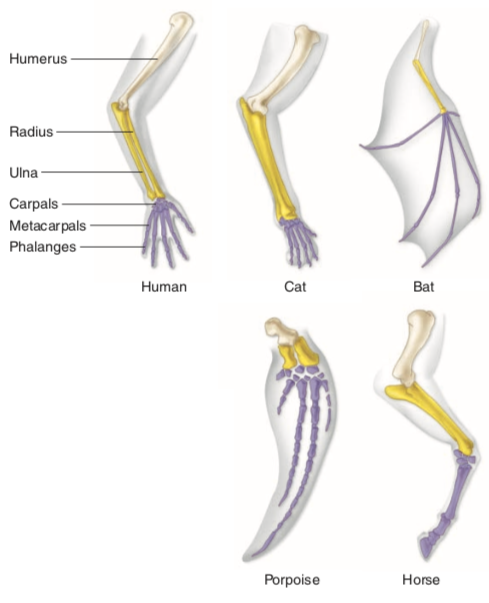
\includegraphics[scale=1.3]{homo}
    \caption{Homologous structure in mammal forearms}
    \label{fig:homo}
\end{figure}

\begin{figure}[h]
    \centering
    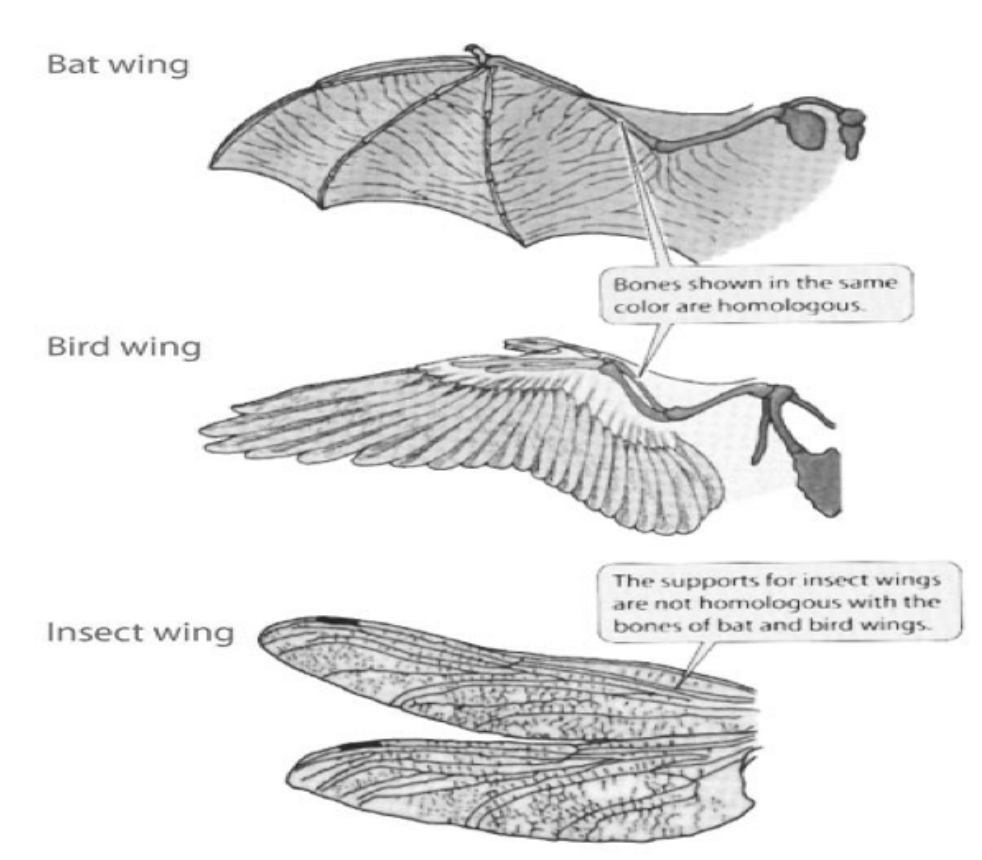
\includegraphics[scale=0.4]{analo}
    \caption{Analogous wing structures in bats, birds, and insects from Google Images}
    \label{fig:analo}
\end{figure}

\paragraph{Homology from genetic information}
Regarding the universality of the genetic code, a simple thought experiment was given by \citeA{Ridley}.
It is known that tRNAs are responsible for the delivery of specific amino acids to the ribosome for protein synthesis.
There are mechanisms in which animo acids bind to the right tRNA.
Suppose there were more than one origins of genetic codes and all were equally competent, since all follow the same chemical mechanism.
The observation that there is only one observed genetic code suggests otherwise.
The only reasonable conclusion is that there must be a single competent origin of the genetic code.

\section{Complexity behind selection}
At this point, it can be summarized that natural selection is a solid mechanism to explain evolution.
Following the above cases on HIV and melanism, the complexity behind interactions has been placed under the term ``natural selection''.
As noted above, natural selection accounts for the complex mechanisms behind natural self-organization in favor of a species variant.
Natural selection is a form of self-organization in the sense that the final allele distribution and niche selection are stable in the long-term.

Carefully following the theory of evolution, it is sufficient to conclude that life has evolved from a single population, and complex interactions with the environment provided the mechanisms for evolution, such as genetic drift and natural selection.
